\documentclass{standalone}
\usepackage{graphicx}	
\usepackage{amssymb, amsmath}
\usepackage{color}

\usepackage{tikz}
\usetikzlibrary{intersections, backgrounds, math}
\usepackage{pgfmath}

\definecolor{light}{RGB}{220, 188, 188}
\definecolor{mid}{RGB}{185, 124, 124}
\definecolor{dark}{RGB}{143, 39, 39}
\definecolor{highlight}{RGB}{180, 31, 180}
\definecolor{light_teal}{RGB}{107, 142, 142}
\definecolor{mid_teal}{RGB}{72, 117, 117}
\definecolor{dark_teal}{RGB}{29, 79, 79}
\definecolor{gray10}{gray}{0.1}
\definecolor{gray20}{gray}{0.2}
\definecolor{gray30}{gray}{0.3}
\definecolor{gray40}{gray}{0.4}
\definecolor{gray60}{gray}{0.6}
\definecolor{gray70}{gray}{0.7}
\definecolor{gray80}{gray}{0.8}
\definecolor{gray90}{gray}{0.9}
\definecolor{gray95}{gray}{0.95}

\begin{document}

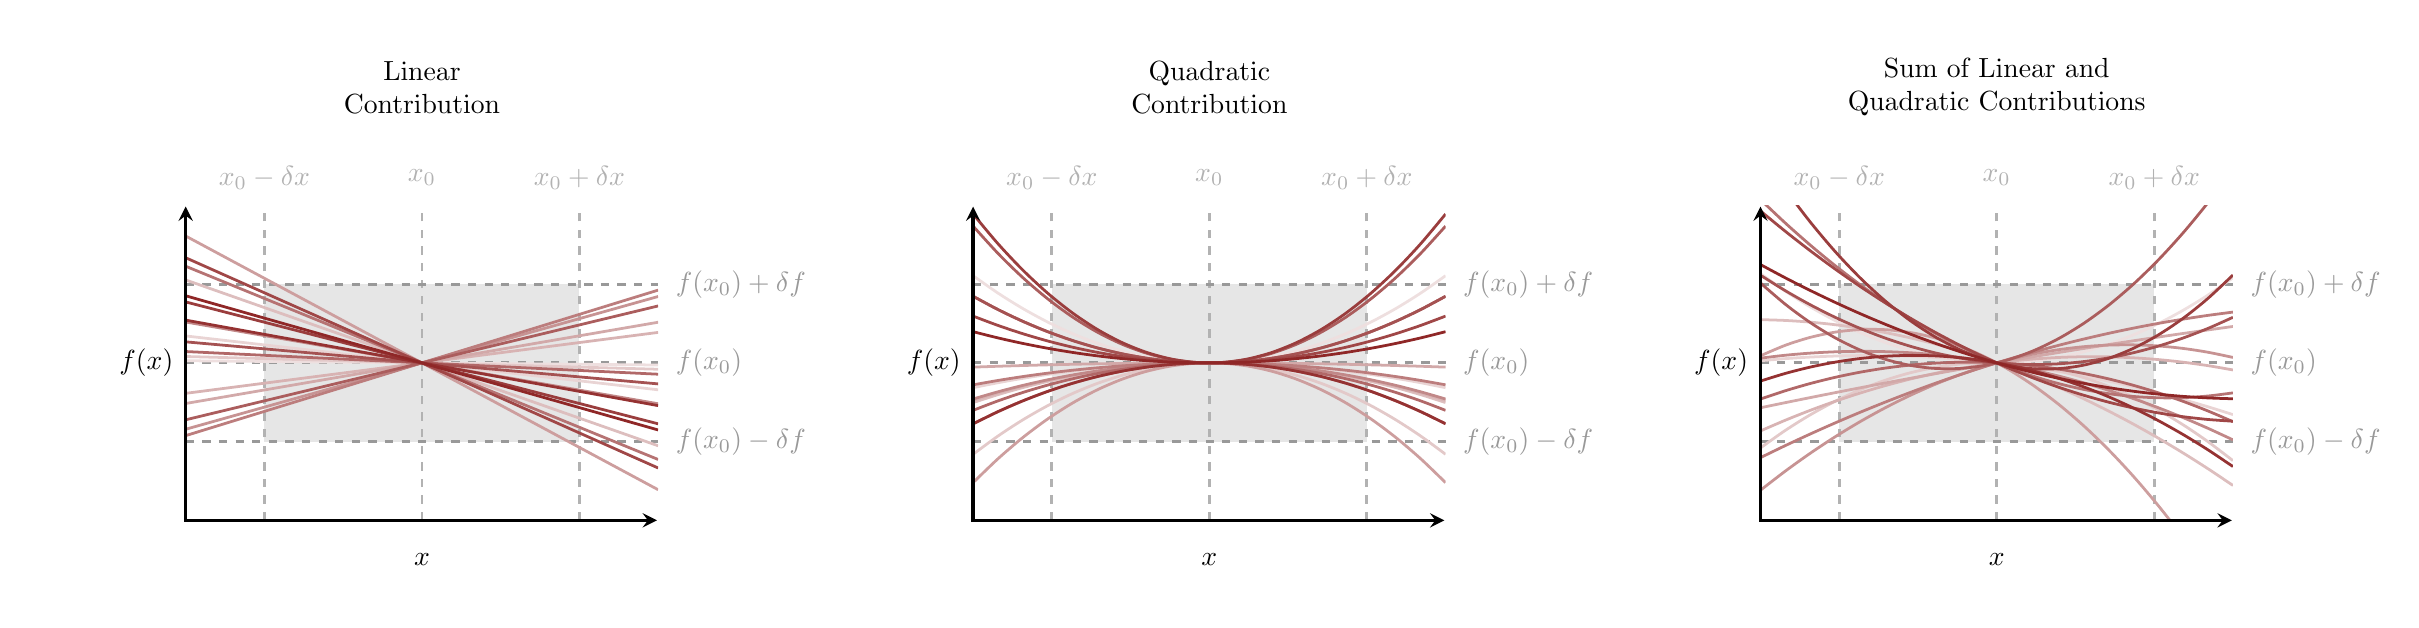
\begin{tikzpicture}[scale=1.0]

  \begin{scope}[shift={(0, 0)}]
    \draw[white] (-5, -3) rectangle (5, 4.25);
    
    \node[align=center] at (0, 3.5) { Linear\\Contribution };
    
    \pgfmathsetmacro{\xo}{0.0};
        
    \fill[gray70, opacity=0.33] (\xo - 2, -1) rectangle (\xo + 2, 1);
    \draw[gray70, dashed, line width=1] (\xo + 2, -2) -- (\xo + 2, 2);
    \draw[gray70, dashed, line width=1] (\xo, -2) -- (\xo, 2);
    \draw[gray70, dashed, line width=1] (\xo - 2, -2) -- (\xo - 2, 2);
    \node[gray70] at (\xo, 2.35) { $x_{0}$ };
    \node[gray70] at (\xo - 2, 2.35) { $x_{0} - \delta x$ };
    \node[gray70] at (\xo + 2, 2.35) { $x_{0} + \delta x$ };

    \draw[gray60, dashed, line width=1] (-3, -1) -- (3, -1);    
    \draw[gray60, dashed, line width=1] (-3, 0) -- (3, 0);
    \draw[gray60, dashed, line width=1] (-3, 1) -- (3, 1);
    
    \node[gray60, anchor=west] at (3.1, -1) { $f(x_{0}) - \delta f$ };    
    \node[gray60, anchor=west] at (3.1, 0)  { $f(x_{0})$ };
    \node[gray60, anchor=west] at (3.1, 1)  { $f(x_{0}) + \delta f$ };
    
    \begin{scope}
      \clip (-3, -2) rectangle (3, 2);
      \foreach \beta [count=\n] in {-0.009, -0.114, -0.027, 
                                    -0.351, 0.129, 0.172, 
                                    -0.537, 0.281, -0.173, 
                                    0.308, -0.409, -0.048, 
                                    0.241, -0.089, -0.445, 
                                    -0.258, -0.181, -0.284} {
        \pgfmathsetmacro{\prop}{5 * \n + 10)};
        \colorlet{custom}{dark!\prop!white};
        \draw[domain={-3:3}, smooth, samples=20, line width=1, variable=\x, color=custom] 
          plot ({\x},{\beta * \x});
      }
    \end{scope}
        
    \draw [->, >=stealth, line width=1.25] (-3.00, -2.015) -- +(0, 4);
    \draw [->, >=stealth, line width=1.25] (-3.015, -2.00) -- +(6, 0);
    
    \node at (-3.5, 0) { $f(x)$ };
    \node at (0, -2.5) { $x$ };
  \end{scope}

  \begin{scope}[shift={(10, 0)}]
    \draw[white] (-5, -3) rectangle (5, 4.25);
    
    \node[align=center] at (0, 3.5) { Quadratic\\Contribution };
    
    \pgfmathsetmacro{\xo}{0.0};
        
    \fill[gray70, opacity=0.33] (\xo - 2, -1) rectangle (\xo + 2, 1);
    \draw[gray70, dashed, line width=1] (\xo + 2, -2) -- (\xo + 2, 2);
    \draw[gray70, dashed, line width=1] (\xo, -2) -- (\xo, 2);
    \draw[gray70, dashed, line width=1] (\xo - 2, -2) -- (\xo - 2, 2);
    \node[gray70] at (\xo, 2.35) { $x_{0}$ };
    \node[gray70] at (\xo - 2, 2.35) { $x_{0} - \delta x$ };
    \node[gray70] at (\xo + 2, 2.35) { $x_{0} + \delta x$ };

    \draw[gray60, dashed, line width=1] (-3, -1) -- (3, -1);    
    \draw[gray60, dashed, line width=1] (-3, 0) -- (3, 0);
    \draw[gray60, dashed, line width=1] (-3, 1) -- (3, 1);
    
    \node[gray60, anchor=west] at (3.1, -1) { $f(x_{0}) - \delta f$ };    
    \node[gray60, anchor=west] at (3.1, 0)  { $f(x_{0})$ };
    \node[gray60, anchor=west] at (3.1, 1)  { $f(x_{0}) + \delta f$ };
    
    \begin{scope}
      \clip (-3, -2) rectangle (3, 2);
      \foreach \beta [count=\n] in {0.123, -0.035, -0.129, 
                                    -0.056, -0.053, -0.006, 
                                    -0.169, -0.086, -0.051, 
                                    -0.031, 0.094, -0.067, 
                                    0.193, 0.094, 0.066, 
                                    0.210, -0.086, 0.044} {
        \pgfmathsetmacro{\prop}{5 * \n + 10)};
        \colorlet{custom}{dark!\prop!white};
        \draw[domain={-3:3}, smooth, samples=20, line width=1, variable=\x, color=custom] 
          plot ({\x},{\beta * \x * \x});
      }
    \end{scope}
        
    \draw [->, >=stealth, line width=1.25] (-3.00, -2.015) -- +(0, 4);
    \draw [->, >=stealth, line width=1.25] (-3.015, -2.00) -- +(6, 0);
    
    \node at (-3.5, 0) { $f(x)$ };
    \node at (0, -2.5) { $x$ };
  \end{scope}

  \begin{scope}[shift={(20, 0)}]
    \draw[white] (-5, -3) rectangle (5, 4.25);
    
    \node[align=center] at (0, 3.5) { Sum of Linear and\\Quadratic Contributions };
    
    \pgfmathsetmacro{\xo}{0.0};
        
    \fill[gray70, opacity=0.33] (\xo - 2, -1) rectangle (\xo + 2, 1);
    \draw[gray70, dashed, line width=1] (\xo + 2, -2) -- (\xo + 2, 2);
    \draw[gray70, dashed, line width=1] (\xo, -2) -- (\xo, 2);
    \draw[gray70, dashed, line width=1] (\xo - 2, -2) -- (\xo - 2, 2);
    \node[gray70] at (\xo, 2.35) { $x_{0}$ };
    \node[gray70] at (\xo - 2, 2.35) { $x_{0} - \delta x$ };
    \node[gray70] at (\xo + 2, 2.35) { $x_{0} + \delta x$ };

    \draw[gray60, dashed, line width=1] (-3, -1) -- (3, -1);    
    \draw[gray60, dashed, line width=1] (-3, 0) -- (3, 0);
    \draw[gray60, dashed, line width=1] (-3, 1) -- (3, 1);
    
    \node[gray60, anchor=west] at (3.1, -1) { $f(x_{0}) - \delta f$ };    
    \node[gray60, anchor=west] at (3.1, 0)  { $f(x_{0})$ };
    \node[gray60, anchor=west] at (3.1, 1)  { $f(x_{0}) + \delta f$ };
    
    \begin{scope}
      \clip (-3, -2) rectangle (3, 2);
      \foreach \betaone/\betatwo [count=\n] in {-0.009/0.123, -0.114/-0.035, -0.027/-0.129, 
                                                -0.351/-0.056, 0.129/-0.053, 0.172/-0.006, 
                                                -0.537/-0.169, 0.281/-0.086, -0.173/-0.051, 
                                                0.308/-0.031, -0.409/0.094, -0.048/-0.067, 
                                                0.241/0.193, -0.089/0.094, -0.445/0.066, 
                                                -0.258/0.210, -0.181/-0.086, -0.284/0.044} {
        \pgfmathsetmacro{\prop}{5 * \n + 10)};
        \colorlet{custom}{dark!\prop!white};
        \draw[domain={-3:3}, smooth, samples=20, line width=1, variable=\x, color=custom] 
          plot ({\x},{\betaone * \x + \betatwo * \x * \x});
      }
    \end{scope}
        
    \draw [->, >=stealth, line width=1.25] (-3.00, -2.015) -- +(0, 4);
    \draw [->, >=stealth, line width=1.25] (-3.015, -2.00) -- +(6, 0);
    
    \node at (-3.5, 0) { $f(x)$ };
    \node at (0, -2.5) { $x$ };
  \end{scope}
  
\end{tikzpicture}

\end{document}  